\chapter{Marco teórico}
Con el desarrollo del sistema producto del presente trabajo terminal se involucran ciertos conceptos provenientes en su mayoría de ramas de ciencias de la computación y en general en alusión a la Inteligencia Artificial, por lo que es conveniente dar contexto sobre los elementos necesarios para el desarrollo del trabajo terminal.
\section{Análisis de Imágenes}
        El análisis de imágenes comprende un conjunto de operaciones sobre una o varias imágenes con el propósito de obtener una imagen con mayor realce o para extraer características útiles, es un tipo de dispensación de señales en el que la entrada es una imagen y la salida puede ser otra imagen o características asociadas a la imagen, algunos de los pasos generales se describen a continuación:
        
        \subsection{Preprocesamiento}
            Preprocesamiento es un nombre común para operaciones con imágenes al más bajo nivel de abstracción. Tanto entrada como salida son imágenes de intensidad. Estas imágenes tienen el mismo tipo de datos que la original, con una imagen de intensidad usualmente representada por una matriz de valores de función de imagen (Brillo) El objetivo de preprocesar es la mejora de los datos de la imagen que borre distorciones o realce características importantes para procesamiento posterior, incluso las transformaciones geométricas de las imagenes e.g (rotación, escalamiento y traslación) son también clasificadas como métodos de preprocesamiento, ya que técnicas similares son utilizadas \cite{imgAnalySeg}.
               
                
        \subsection{Realce de la imagen}
            El objetivo principal de realce de imagen es también procesar una imagen dada tal que el resultado sea mas ajustable que la imagen original para aplicaciones específicas. Por ejemplo para la remoción de ruido.
            \\\\%\bigskip
            Acentúa o afina características de la imagen como ejes, límites o contraste para hacer un despliegue gráfico mas útil para el análisis.
            \\\\%%\bigskip
            El realce no incrementa o decrementa el contenido de la información inherente de los datos pero sí incrementa el rango dinámico de las características elegidas de tal modo que puedan ser detectadas fácilmente.
            \\\\%\bigskip
            Proveé \'mejor\' entrada para otras técnicas avanzadas de procesamiento automatizadas de imágenes.
                        
        \subsection{Segmentación de la imagen}
            El término segmentación utilizada en el contexto de análisis de imágenes se refiere a la partición de una imagen en un conjunto de regiones que la cubren. El objetivo en muchas de las tareas es que para las regiones se representen áreas significativas de la imagen, como áreas urbanas, fronteras o bosques de una imagen satelital. En otras tareas de análisis, las regiones pueden ser conjuntos de bordes de pixeles agrupados en estructuras como segmentos de líneas y segmentos de arcos circulares en imágenes de objetos industriales en 3D. Las regiones pueden también estar definidas como grupos de pixeles teniendo ambos un borde y una forma particular como un circulo o una elipse or polígono. Cuando las regiones de interés no cubren la imagen completa, aún se requiere el proceso de segmentación en regiones de y de fondo para ignorarse. 
            \cite{imgAnalySeg}
            %REF courses.cs.washington.edu/courses/cse576/book/ch10.pdf
            \begin{figure}[H]
                \centering
                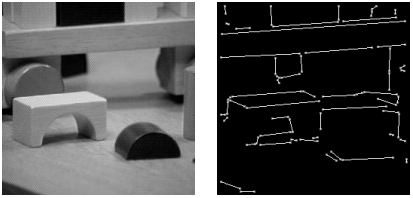
\includegraphics[width=0.7\textwidth]{capitulo2/images/segmentation.PNG}
                \caption{Imagen con bloques (Izquierda) y conjunto de segmentos de linea extraídos (Derecha).}
                \label{fig:segmentacion}
            \end{figure}
        %\subsection{Extracción de características}
            
            %http://citeseerx.ist.psu.edu/viewdoc/download?doi=10.1.1.375.6848&rep=rep1&type=pdf
        %\subsection{Clasificación e interpretación}
            %http://citeseerx.ist.psu.edu/viewdoc/download?doi=10.1.1.375.6848&rep=rep1&type=pdf


\section{Métodos de reconocimiento de expresiones matemáticas}
\subsection{Análisis sintáctico dirigido}
Los lenguajes libres de contexto, son aquellos que tienen una notación recursiva natural llamada \textit{gramática libre de contexto}. Por ende, un lenguaje libre de contexto es todo aquel que puede ser representado por una gramática libre de contexto.

Una gramática libre de contexto G, queda definida de la siguiente manera:

\begin{equation}
    G = (V, T, P, S)
\end{equation}

de donde, V es el conjunto de variables, T el conjunto de símbolos terminales, P el conjunto de producciones y S el punto de inicio \cite{automata}.

El lenguaje matemático, es decir, las expresiones matemáticas son un lenguaje libre de contexto. Esto quiere decir que es posible definir una gramática libre de contexto para definir a las expresiones matemáticas. Esta es una práctica muy común en la teoría de compiladores.

Sabiendo esto, una aproximación a la resolución del problema de reconocer expresiones matemáticas en imágenes es la que describe \cite{gramaticasAnderson}. El método consiste en dos etapas:

\begin{itemize}
    \item Reconocimiento de caracteres: Utilizar algún método de reconocimiento de patrones para localizar los caracteres y anotar sus coordenadas. 
    \item Análisis sintáctico dirigido: Utilizar la etapa previa para determinar la jerarquía, basándose en un conjunto de reglas definidas (las gramáticas libres de contexto).
\end{itemize}

En la Figura \ref{fig:gramaticas}, se puede ver un ejemplo del proceso de reconocimiento propuesto por este método.

\begin{figure}[h]
    \centering
    \subfigure[]{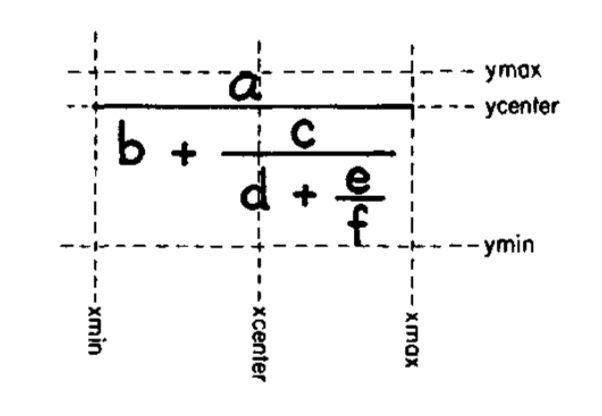
\includegraphics[width=6cm]{capitulo2/images/gramaticas1}}
    \subfigure[]{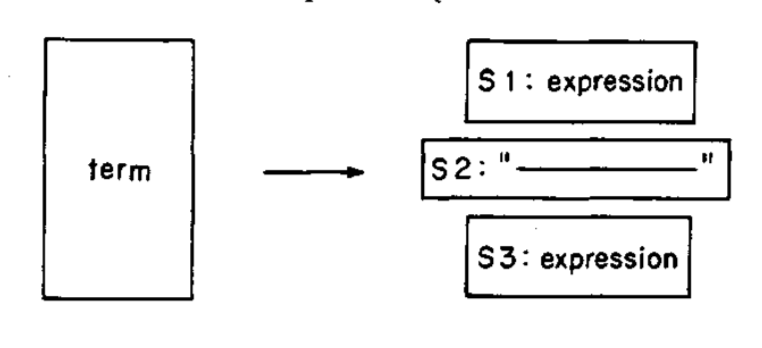
\includegraphics[width=6cm]{capitulo2/images/gramaticas2}}
    \caption{\textbf{a)} La primera etapa del método de reconocimiento, se anotan las coordenadas de de cada caracter. \textbf{b)} Se realiza un análisis sintáctico con las gramáticas libres de contexto definidas.}
    \label{fig:gramaticas}
\end{figure}

\newpage
\subsection{Redes Neuronales}
    Existe un tipo de neurona artificial llamada perceptrón desarrolladas entre 1950 y 1960 por el científico Frank Rosenblatt, sin embargo este modelo ha ido evolucionando y hoy en día se utilizan otros modelos de neurona como el llamado sigmoid neuron, que para entender, primero se debe definir al perceptrón como modelo.
    Un perceptrón toma varias entradas binarias $x_{1},x_{2},x_{3},...,x_{n}$ y produce una sola salida binaria:
     \begin{figure}[H]
        \centering
        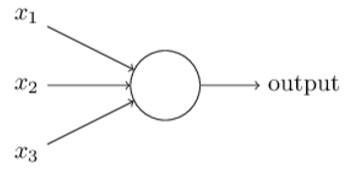
\includegraphics[width=0.5\textwidth]{capitulo2/images/perceptron.PNG}
        \caption{Representación de un percetrón con entradas $x_{1}$, $x_{2}$ y $x_{3}$}
        \label{fig:perceptron}
    \end{figure}
    La regla que Rosenblatt introdujo para calcular la salida involucra valores llamados pesos $w_{1},w_{2},w_{3},...$ que pueden tomar valores reales expresando la importancia de las respectivas entradas a la salida, la salida de la neurona (0 o 1) es determinado por la suma ponderada $\sum_{j} w_{j} x_{j}$ es menor o igual a un valor de umbral. Así como los pesos, el valor de umbral es un número real el cuál es un parámetro de la neurona:
     \begin{equation}
        output = \left\{ \begin{array}{lcc}
             0 &   si  & \sum_{j} w_{j} x_{j} \leq threshold \\
             \\ 1 &  si & \sum_{j} w_{j} x_{j} \ge threshold\\
             \end{array}
        \right.
    \end{equation}
    \newpage
    Una red neuronal es una red de perceptrones que agrega complejidad a las decisiones.
    \begin{figure}[H]
        \centering
        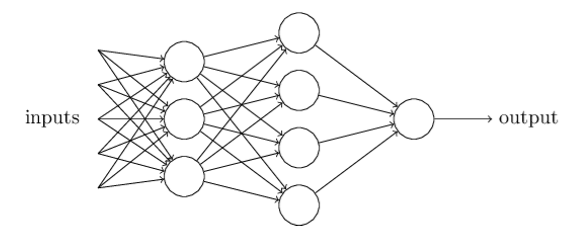
\includegraphics[width=1\textwidth]{capitulo2/images/NNmodel.PNG}
        \caption{Red neuronal de 3 capas}
        \label{fig:NNmodel}
    \end{figure}
    \subsubsection{Conjunto de entrenamiento}
    El conjunto de entrenamiento es un conjunto de datos que se utiliza a modo de ejemplo para que un modelo pueda aprender. En el aprendizaje supervisado el conjunto de entrenamiento se compone de muchas tuplas (X,Y) siendo X un vector de características del problema y Y un vector del resultado al que queremos llegar \cite{deeplearningbook}.
    
    
    \subsubsection{Aprendizaje Profundo}
        El aprendizaje profundo de forma clásica se refiere al tratamiento de redes neuronales con mas de dos capas, sin embargo, debido al cambio que esta sub-area ha sufrido, se debe definir como el tratamiento de redes neuronales con un largo número de parámetros y capas en una de las cuatro arquitecturas de redes fundamentales:
        \begin{itemize}
            \item Redes pre-entrenadas no supervisadas
            \item Redes Neuronales Convolucionales
            \item Redes neuronales recurrentes
            \item Redes neuronales recursivas.
        \end{itemize}
    
    Siendo las Redes Neuronales Convolucionales de las que se expondrá a detalle en  \\%siguiente subseccion.
    \\Una de las propiedades mas importantes que permite el Aprendizaje Profundo es la extracción automática de características que puede ser clave en dicho paso del análisis de imágenes.
    
    \subsubsection{Redes Neuronales Convolucionales}
    Las redes neuronales convolucionales han ganado popularidad en los últimos años debido a su efectividad prometedora en el aprendizaje profundo. Partiendo por el procesamiento de imágenes, las capas convolucionales han encontrado su camino en otros subcampos del aprendizaje profundo y muestran éxito en la mayor parte de dichos campos.\\\\ 
    La diferencia fundamental entre \textit{fully connected} (completamente conectadas) y \textit{convolutional neural networks}(redes neuronales convolucionales) es el patrón de conexión entre las capas consecutivas. En el caso de las completamente conectadas como el nombre lo sugiere, cada unidad es conectada a todas las unidades de la previa capa. \\\\
    En una capa convolucional de una red neuronal, por otra parte, cada unidad está conectada a (típicamente pequeña) un número de unidades cercanas en la capa previa. Más aún, todas las unidades están conectadas a la capa previa de la misma forma con los pesos exactamente iguales y estructura. Esto lleva a una operación conocida como convolución, dando a la arquitectura este nombre, a grandes rasgos esto significa aplicar una pequeña "ventana" de pesos (conocida como filtro) sobre una imágen como se muestra en la figura \ref{fig:CNNFilter}.
    
    
     \begin{figure}[H]
        \centering
        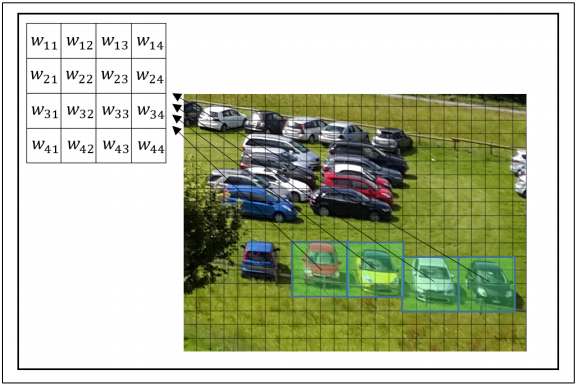
\includegraphics[width=0.7\textwidth]{capitulo2/images/CNN_window.png}
        \caption{Matriz de pesos conocida como ventana aplicada a una imagen.}
        \label{fig:CNNFilter}
    \end{figure}
    \newpage
    
   
  
    \subsubsection{Arquitectura Encoder-Decoder}
    
    En particular se discutirá la arquitectura de Long Short-Term Memory (LSTM). LSTM es una arquitectura de una red neuronal recurrente diseñada para resolver problemas secuenciales, normalmente conocidos como sequence-to-sequence. Los problemas secuenciales, tienen usualmente como reto, predecir el siguiente resultado encontrado. Un reto que surge naturalmente de estos problemas, es la longitud variable de las entradas.
    
    Una aproximación para resolver los problemas secuenciales es el Encoder-Decoder LSTM él cual ha probado ser efectivo en muchos casos. Esta arquitectura se compone de dos modelos \cite{encoderDecoder}:
    
    \begin{itemize}
    	\item Encoder: Es una red neuronal encargada de leer la entrada de longitud variable y convertirla en un vector de longitud fija.
    	\item Decoder: Es una red neuronal encargada de tomar la salida del Encoder y como salida obtiene un valor predecido.
    \end{itemize} 


	\subsubsection{Image Captioning}
    
    Es una rama emergente del \textit{deep learning} que ha ido ganando atención en los últimos años. Este campo es un punto intermedio entre la vision por computadora y el procesamiento del lenguaje natural. El actual estado del arte en image captioning tiene una aproximación similar a los modelos sequence-to-sequence, los cuales utilizan una arquitecura Encoder-Decoder \cite{imagetolatex}.
    
    Si se trata al problema de reconocer expresiones matemáticas en imagenes como un problema sequence-to-sequence de image captioning, se puede emplear una arquitectura de Encoding-Decoding para hacer la conversión de la imagen a LaTeX de manera directa. Esto permite a la red manejar imagenes de longitud variable y reconocer los símbolos a la vez que va reconociendo las expresiones.
    
    La arquitectura que se esta utilizando actualmente para solucionar este problema se muestra en la Figura \ref{fig:imgcaptioning} \cite{imagetolatex}\cite{imagemarkup}\cite{chino}.
    
    \begin{figure}
		\centering
		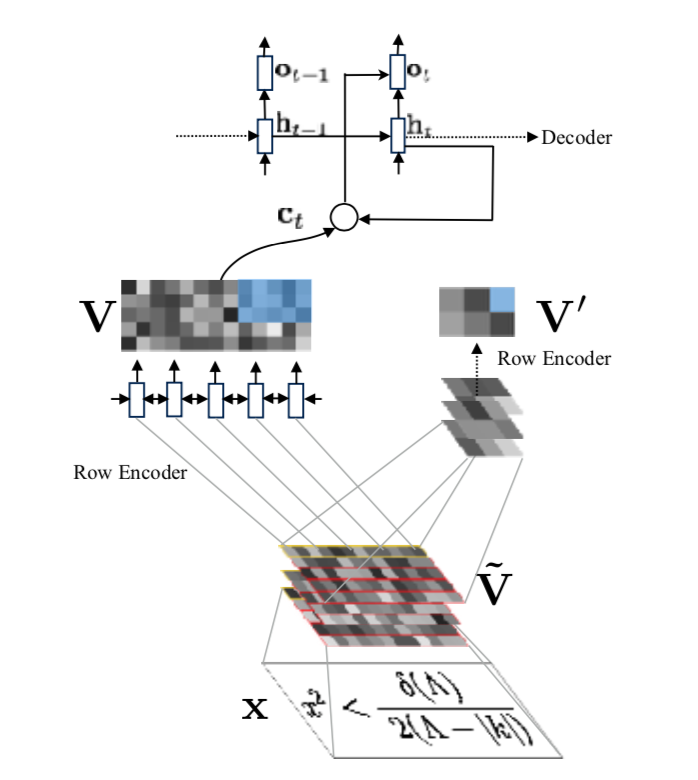
\includegraphics[width=8cm]{capitulo2/images/imgcaptioning}
		\caption{Arquitectura de image captioning para reconocer expresiones matemáticas en imagenes.}
		\label{fig:imgcaptioning}
    \end{figure}

\subsection{Análisis estructural}

Este método coincide con el primero en que debe de utilizar una técnica de reconocimiento de patrones para etiquetar primero los símbolos. Las etiquetas que utiliza tienen que ver son su posición en la imagen, así como su tamaño. 

La diferencia en este método, radica en su segunda etapa. No se realizará un análisis con gramáticas, en su lugar se intentara deducir la estructura jerárquica con algún otro método. El artículo \cite{spanningtree} propone utilizar el algoritmo de Kruskal para obtener un árbol de recubrimiento mínimo por niveles, de este modo se puede saber la estructura de la expresión matemática recorriendo el gráfo resultante.La Figura \ref{fig:spanningtree} muestra un ejemplo de como funciona este método.

\begin{figure}[h]
	\centering
	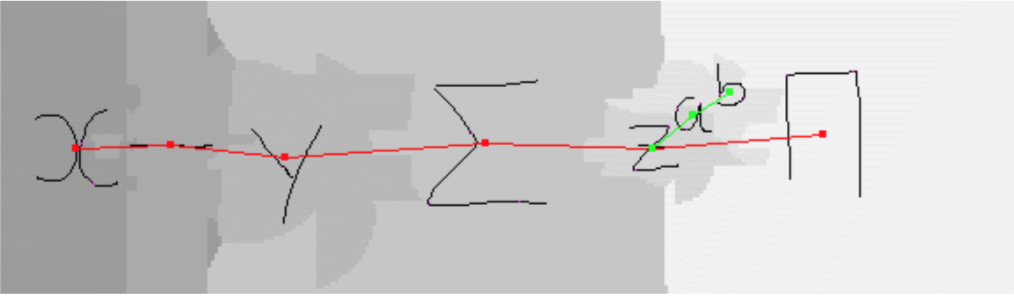
\includegraphics[width=8cm]{capitulo2/images/spanningtree}
	\caption{Utilización de un árbol de recubrimiento mínimo para el reconocimiento de expresiones matemáticas.}
	\label{fig:spanningtree}
\end{figure}
\newpage
\subsection{Aprendizaje profundo como servicio}
El entrenamiento de redes neuronales profundas, conocidas como aprendizaje profundo es en la actualidad áltamente complejo computacionalmente. Requiere un sistema con la combinación correcta de software, drivers, memoria, red y recursos de almacenamiento, por factores como estos los proveedores de cloud computing como Amazon Web Services, Microsoft Azure o Google Cloud ofrecen actualmente servicios de Machine Learning proveyendo API's como pueden ser de entrenamiento de modelos o de visualización de datos y generación de estadísticas, permitiendo que desarrolladores y científicos de datos se enfoquen mas en tareas como el entrenamiento de modelos, análisis de datos, etc.
\\\\
Los modelos de aprendizaje profundo requieren de un proceso experimental e iterativo, requiriendo cientos e incluso miles de ejecuciones que requieren de un amplio poder de cómputo para encontrar la combinación correcta de las configuraciones e hiper-parámetros de la red neuronal. Esto puede tomar semanas o incluso meses y este tipo de servicios garantiza una disponibilidad en todo momento y en conjunto permite que un sistema completo esté dividido en módulos consiguiendo que el mantenimiento y detección de fallos sean tareas más sencillas.
\\\\ 
En la figura \ref{fig:DLAAS} se puede observar la arquitectura de un sistema divido en módulos y que hace uso de herramientas de Machine Learning para dar respuesta a otros módulos del sistema.

\begin{figure}[H]
	\centering
	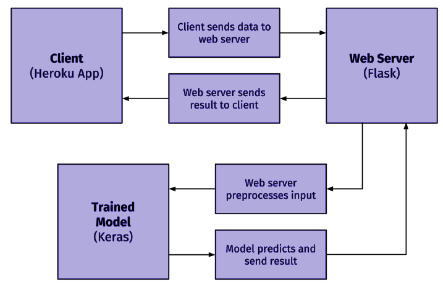
\includegraphics[width=0.7\textwidth]{capitulo2/images/DLAAS.png}
	\caption{Ejemplo de sistema con módulo de Machine Learning}
	\label{fig:DLAAS}
\end{figure}    


\section{Aplicación web}
En la ingeniería de software se denomina aplicación web a aquellas herramientas que los usuarios pueden utilizar accediendo a un servidor web a través de internet o de una intranet mediante un navegador. En otras palabras, es un programa que se codifica en un lenguaje interpretable por los navegadores web en la que se confía la ejecución al navegador \cite{appweb}.

\subsection{Django}
Django es un framework de desarrollo web completamente desarrollado en Python. Permite de una manera rápida poder implementar una aplicación web en el lenguaje Python. Las siguientes, son de las principales características de Django:

\begin{itemize}
    \item \textbf{Rápido}: Tiene como filosofía ayudar a los desarrolladores a crear aplicaciones en el menor tiempo posible.
    \item \textbf{Completo}: Incluye cientos de librerías que permiten ahorrar tiempo y automatizar tareas.
    \item \textbf{Seguro}: Es una de las principales características de Django ya que incluye soluciones a los principales ataques que puede sufrir una aplicación web.
    \item \textbf{Escalable}: Con el patrón de diseño de Django es posible incrementar o decrementar la capacidad de un sitio.
    \item \textbf{Versátil}: Es utilizado por muchas empresas y organizaciones a lo largo del mundo para crear diferentes tipos de proyectos.
\end{itemize}

\subsubsection{Modelo-Vista-Template}
El Modelo-Vista-Template (MTV) es el patrón de diseño que Django implementa. Este patrón es una modificación al conocido Modelo-Vista-Controlador (MVC). La diferencia radica en que Django se encarga de hacer la parte del controlador, por ende el desarrollador solamente tiene que preocuparse por implementar la lógica de negocio y de como mostrará los datos. En la Figura \ref{fig:mtv}, se puede ver una representación del patrón MTV. En el patrón de diseño MTV \cite{mtv}:

\begin{figure}
    \centering
    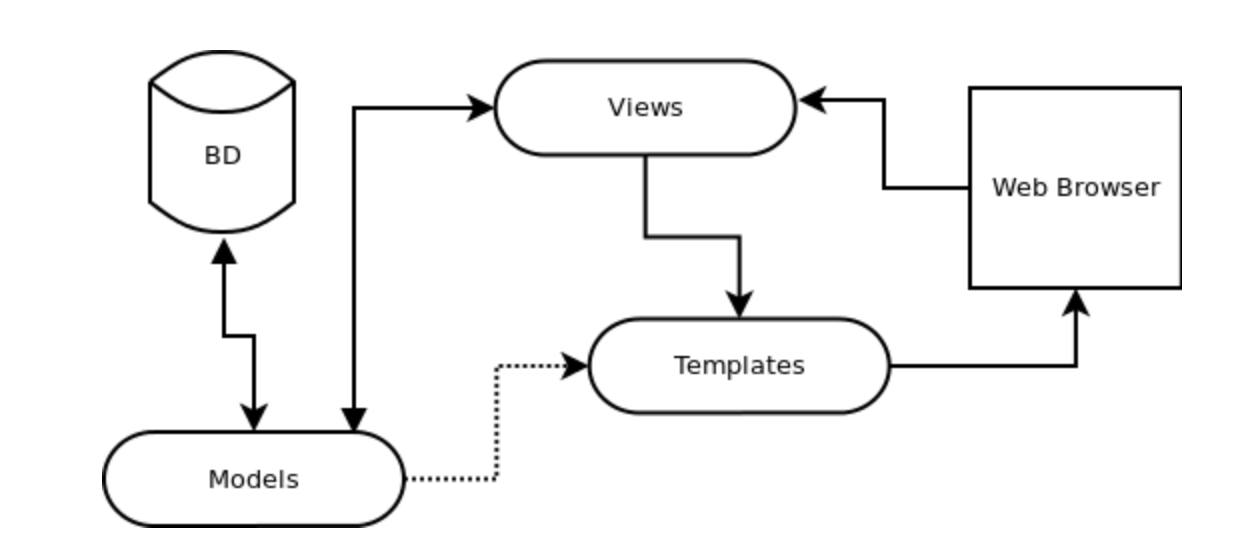
\includegraphics[width=\textwidth]{capitulo2/images/mtv.png}
    \caption{Representación del patrón de diseño Modelo-Vista-Template.}
    \label{fig:mtv}
\end{figure}

\begin{itemize}
    \item \textbf{Modelo}: La capa de acceso a la base de datos. Esta capa contiene toda la información sobre los datos: cómo acceder a estos, cómo validarlos, cuál es el comportamiento que tiene, y las relaciones entre los datos.
    \item \textbf{Template}: La capa de presentación. Esta capa contiene las decisiones relacionadas a la presentación: como algunas cosas son mostradas sobre una página web o otro tipo de documento.
    \item \textbf{Vista}: La capa de la lógica de negocios. Esta capa contiene la lógica que accede al modelo y la delega a la plantilla apropiada: puedes pensar en esto como un puente entre el modelos y las plantillas.
\end{itemize}

\subsection{API REST}
\subsubsection{Application Programming Interface}
Una Interfaz de Programación de Aplicaciones o API es un conjunto de definiciones y protocolos que se utilizan para desarrollar e integrar el software de las aplicaciones.

Las API permiten que sus servicios se comuniquen con otros, sin necesidad de saber como están implementados. Esto simplifica el desarrollo de las aplicaciones y permite ahorrar tiempo y dinero \cite{apiArticle}.
\subsubsection{Represenational State Transfer}

Representational State Transfer (REST) es un estilo de arquitectura basado en un conjunto de principios que describen como recursos interconectados son definidos y direccionados. Estos principios fueron descritos en el año 2000 por Roy Fielding como parte de obtención de su doctorado.
\\
Es importante hacer énfasis en que REST es un \textbf{estilo de software de arquitectura} y no un conjunto de estandares. Como resultado, dichas aplicaciones o arquitecturas son en ocasiones referidas como aplicaciones RESTful o REST-style \cite{restArticle}. 
\\
Una aplicación o arquitectura considerada RESTful o REST-style es caracterizada por:
\begin{itemize}
	\item La funcionalidad y estado son dividiad en recursos distribuidos.
	\item Cada recurso es únicamente direccionable usando un conjunto uniforme y mínimo de comandos (típicamente usando comandos HTTP de GET, POST, PUT o DELETE).
	\item El protocolo es cliente/servidor, stateless, por capas y soporta almacenamiento cache.
\end{itemize} 
 La figura \ref{fig:rest_mess} ilustra el uso de REST para servicios Web.
\begin{figure}[H]
	\centering
	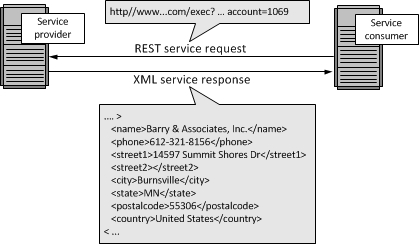
\includegraphics[width=0.5\textwidth]{capitulo2/images/rest_messages.jpg}
	\caption{Consumidor y proveedor de servicios comunicandose mediante solicitudes y respuestas REST.}
	\label{fig:rest_mess}
\end{figure}  
\subsubsection{Autentificación}
Para hablar de autentificación es necesario primero entender la diferencia entre identificación y autentificación, por un lado la identificación es la capacidad de identificar de forma exclusiva a un usuario de un sistema o una aplicación que se está ejecutando, mientras que la autentificación es la capacidad de demostrar que un usuario o una aplicación es quien dicha persona o aplicación asegura ser \cite{authent}.\\\\
Para el caso de una REST API es en muchas ocasiones necesario que se lleve a cabo la autentificación para permitir o denegar el acceso a recursos de un servidor por ejemplo de acuerdo a los permisos concedidos en función de las credenciales de autentificación para así asegurar que los datos sean visibles únicamente a aquellos que proporcionen las credenciales adecuadas y dispongan de los permisos necesarios.

%https://www.ibm.com/support/knowledgecenter/es/SSFKSJ_7.5.0/com.ibm.mq.sec.doc/q009740_.htm
\section{Android}
Esta sección tiene objetivo presentar las principales características en el desarrollo de la aplicación para Android.
\subsection{Arquitectura de la aplicación}
Para el desarrollo de la aplicación se implemento la arquitectura Clean, la cual como ya se ha mencionado antes se ha mencionado se ha vuelto muy popular en el desarrollo de aplicaciones móviles para android debido a que es una solución que produce sistemas que presentan las siguientes características.

\begin{itemize}
    \item Escalables, por lo que se pueden agregar más funcionalidades de forma sencilla.
    \item Presentan modularidad.
    \item Presentan independencia en cuanto a frameworks, interfaz de usuario y bases de datos.
    \item El proyecto es más fácil de mantener por lo que es más sencillo hacer cambios.
\end{itemize}

Al utilizar esta arquitectura el proyecto queda separado en tres capas como se observa en la figura \ref{fig:capas-arquitectura} con lo cual cada una de ellas tiene su propósito definido.

\begin{figure}[h]
    \centering
    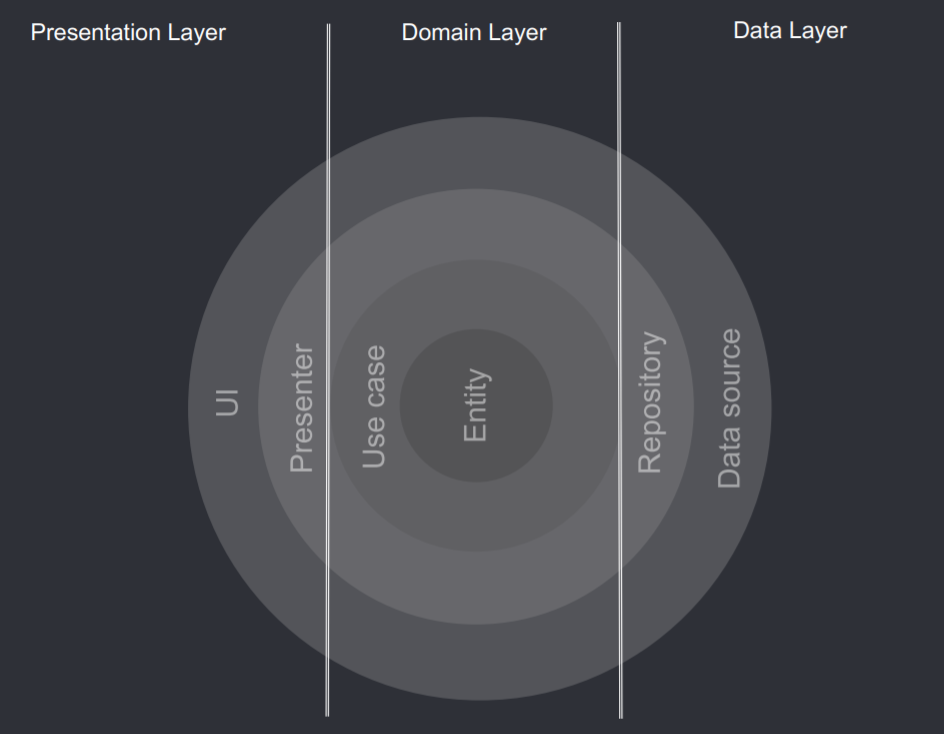
\includegraphics[width=250px]{capitulo5/android/img/capas-clean.png}
    \caption{Tres capas que se tienen al utilizar la arquitectura Clean \cite{cleanGuide}}
    \label{fig:capas-arquitectura}
\end{figure}

\subsubsection{Capa de datos}
La información que se utiliza en el resto de capas proviene de esta capa. Esta capa a su vez se encuentra dividida en la capa de repositorio y en la capa de fuente de datos. 

\paragraph{Capa de repositorio} En esta capa se utiliza el patrón de repositorio como se muestra en la figura \ref{fig:capa-datos}. Gracias a este patrón se puede tener acceso a diferentes fuentes de datos que se encuentran en la capa más baja de nuestra arquitectura, esto nos permite un acceso a los datos de forma transparente para el usuario bajo las condiciones que se presenten.

La forma de utilizar este patrón en la aplicación desarrollado crear una clase en la cual se hace uso de la interfaz que se tiene para el acceso a la fuente de datos. En el siguiente código se puede apreciar el como se crea una instancia de APIService que es nuestra interfaz para fuente de datos.

Después, en nuestro método findAllProyecttosByUser se recupera la información necesaria para mandarla a las capas superiores.

\lstinputlisting[language=Java]{capitulo5/android/src/repositorio.java}

\begin{figure}[h]
    \centering
    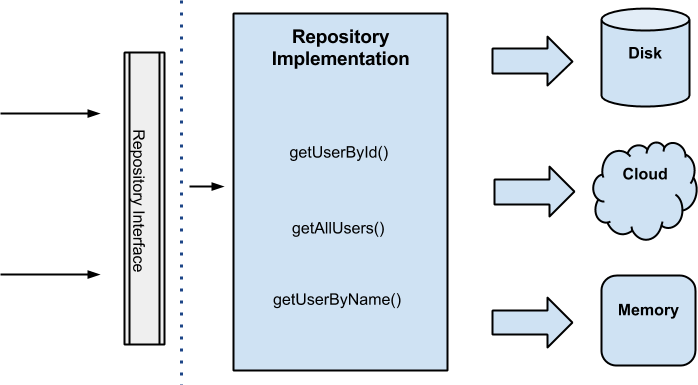
\includegraphics[width=400px]{capitulo5/android/img/capa-datos.png}
    \caption{Capa de datos \cite{cleanWay}}
    \label{fig:capa-datos}
\end{figure}

\paragraph{Capa de fuente de datos} En este trabajo, la fuente de datos que se tiene es un API REST, sin embargo si se requiere acceder a información que se persista en el teléfono se pude agregar otra fuente de datos. Se utilizó retrofit para poder realizar la comunicación con el API REST. 

La forma de utilizar retrofit es crear una interfaz con todos los métodos para recuperar o enviar información al API REST, en esta interfaz cada método tiene la URL a la cual se realizara la petición con alguno de los métodos que tiene HTTP, se tienen los parámetro que se envían y cada método nos regresa una llamada asíncrona que se trabaja en la capa de repositorio. Esto se puede apreciar en el siguiente código.

\lstinputlisting[language=Java]{capitulo5/android/src/APIService.java}

Para poder hacer uso de esta interfaz se tiene que configurar bajo ciertas características especificas como lo son la URL a la cual hará peticiones, el logger que se utilizara para poder observar las peticiones que se realizan y brindar una retroalimentación a la hora de hacer pruebas y por ultimo el parser que se utilizara para trabajar y pasar de clases a datos que el API REST entienda y pueda utilizar, en este caso se utilizo el formato JSON. La definición de estas características se tiene en el siguiente código.

\lstinputlisting[language=Java]{capitulo5/android/src/ServiceGenerator.java}

Finalmente, en esta capa se tienen clases Java que después se mapean a objetos JSON y viceversa, para realizar esto se crea un POJO con los atributos que se necesitan además de agregar anotaciones de retrofit para que el parser pude hacer la conversión necesaria. Un ejemplo de esto es en la siguiente clase de java.

\lstinputlisting[language=Java]{capitulo5/android/src/UsuarioData.java}


\subsubsection{Capa de dominio}
En esta capa es la intermediaria entre las otras dos capas que se tienen, es donde se encuentran los casos de uso también conocidos como interactors como se muestra en la figura \ref{fig:capa-dominio} en ellos la lógica del negocio es ejecutada es por esto que es el núcleo de la aplicación.

Es importante mencionar que esta capa, al ser la encargada del negocio es donde se hacen validaciones en la información y dicha información se adapta para que sea trabajada en la capa de presentación o en la de datos

Además de contener los casos de uso en esta capa se encuentran las entidades y se hace uso de los repositorios para acceder a la información proporcionada por la capa de datos.

\begin{figure}[h]
    \centering
    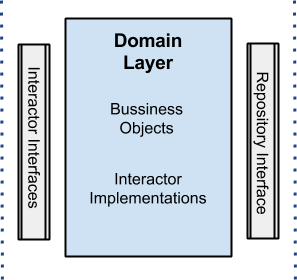
\includegraphics[width=200px]{capitulo5/android/img/capa-dominio.png}
    \caption{Capa de dominio \cite{cleanWay}}
    \label{fig:capa-dominio}
\end{figure}

Para tener un control sobre posibles errores en la capa de presentación o en la capa de datos se utilizan códigos de resultados al igual que una clase que contiene el resultado que se puede presentar, así como la información que se le regresa a la capa de presentación. Se hace uso de genéricos para poder reutilizar esta clase en toda la aplicación y no duplicar código. La clase es la siguiente.

\lstinputlisting[language=Java]{capitulo5/android/src/BusinessResult.java}

La forma en la que se utiliza esta clase en un caso de uso se presenta en el siguiente código que permite iniciar sesión.

\lstinputlisting[language=Java]{capitulo5/android/src/UserInteractorImpl.java}

A su vez el caso de uso utiliza sus propios clases de java para presentar información al usuario en la capa de presentación así como controlar posibles errores en la información que ingrese el usuario los campos de los formularios, un ejemplo de este tipo de clases es el siguiente.

\lstinputlisting[language=Java]{capitulo5/android/src/UsuarioModel.java}

\subsubsection{Capa de presentación}
En esta capa como se muestra en la figura \ref{fig:capa-presentacion} se trabaja con la lógica relacionada a las interfaces que se tienen en la aplicación, es decir a actividades, fragmentos y archivos XML.

\begin{figure}[h]
    \centering
    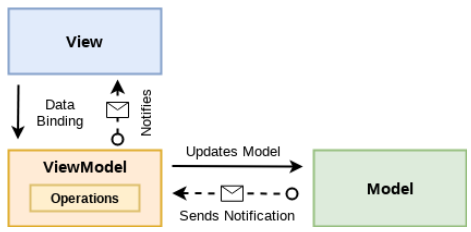
\includegraphics[width=300px]{capitulo5/android/img/capa-presentacion.png}
    \caption{Capa de presentación \cite{cleanWayReload}}
    \label{fig:capa-presentacion}
\end{figure}

En esta capa se pueden trabajar con patrones como MVC y MVP pero en este caso se utiliza el patrón MVVM cada uno con una función en particular. \cite{cleanWayReload}

\begin{itemize}
    \item \textbf{Modelo} Se encarga de representar la información que sera presentada en la vista.
    \item \textbf{Vista} Compuesta en este caso por las actividades y fragmentos de la aplicación, su tarea es mostrar la información, hacen uso de los viewmodels para poder realizar cambios en la interfaz.
    \item \textbf{ViewModel} El ViewModel sera el encargado de ejecutar los casos de uso o interactors con el objetivo de actualizar la vista de acuerdo a la información que presente el modelo.
\end{itemize}


